%% P4 -- Computers & Geosciences (Elsevier) submission draft
%% Manuscript type: research paper
%% Build: pdflatex manuscript ; bibtex manuscript ; pdflatex manuscript ; pdflatex manuscript
%% Supplement: supplement.tex (same chain), excluded from the manuscript word count.
\documentclass[preprint,12pt,authoryear]{elsarticle}

\usepackage{amsmath}
\usepackage{booktabs}
\usepackage{array}
\usepackage{graphicx}
\usepackage{url}

\setlength{\emergencystretch}{2em}

\journal{Computers \& Geosciences}

\begin{document}

\begin{frontmatter}

\title{A dimensionless verification floor for model assessment: which accuracy claims can an observational archive actually resolve?}

\author[1]{[AUTHOR GIVEN NAME] [AUTHOR SURNAME]\corref{cor1}}
\ead{[AUTHOR EMAIL]}
\author[1]{[AUTHOR GIVEN NAME] [AUTHOR SURNAME]}
\author[2]{[AUTHOR GIVEN NAME] [AUTHOR SURNAME]}

\affiliation[1]{organization={[AUTHOR AFFILIATION 1]}}
\affiliation[2]{organization={[AUTHOR AFFILIATION 2]}}

\cortext[cor1]{Corresponding author}

\begin{abstract}
Model assessment compares a simulated field, or an observation-based reference, against independent truth and reports an error metric. Whether the archive can resolve the discrepancy the evaluation is asked to detect is rarely checked, and never in a form comparable across variables. We present a dimensionless method whose inputs are three quantities an assessment already reports: the standard deviation $\sigma_d$ of the product--truth difference, the effective number of independent truth samples $n_{\mathrm{eff}}$, and the magnitude of the asserted claim. It returns $\Phi = 2.802\,\sigma_d/(\mathrm{claim}\sqrt{n_{\mathrm{eff}}}) = \mathrm{MDE}_{80}/\mathrm{claim}$, the ratio of the 80\,\% verification floor to the claim, where the constant encodes a two-sided test at $\alpha = 0.05$ with 80\,\% power and $n_{\mathrm{eff}}$ follows the Kish design effect. The output is a testability index and the largest claim the archive can support; $\Phi>1$ means the claim lies below the floor and cannot be verified, $\Phi<1$ that it can be, not that it is correct. Across five variables the method orders the domains: salinity 0.019, precipitation 0.043, soil moisture 0.24, sea-ice thickness 1.3--3.7 and regional biomass 2.71. For sea ice, whose floor is not a single number, two defensible kernels give 3.447 and 10.38 cm (a factor of 2.5--3.0); the ambiguity is derived in the supplement and carried into the interval. A $\pm 50\,\%$ perturbation of $\sigma_d$ and the claim leaves salinity, precipitation and soil moisture verifiable, sea ice unverifiable at its exponential-kernel bound, and biomass above unity except at the optimistic corner ($\Phi = 0.90$). The boundary is part of the method: one claim at a time, independent truth, and a reported correlation model. $\Phi>1$ says nothing about a study's value, and $\Phi<1$ is necessary but not sufficient -- the SMAP claim has $\Phi = 0.24$ and was met at 18 of 34 sites.
\end{abstract}

\begin{keyword}
verification \sep statistical power \sep effective sample size \sep model assessment \sep sea-ice thickness \sep satellite validation
\end{keyword}

\end{frontmatter}

\section{Introduction}

Model assessment rests on comparisons. A simulated thickness, temperature, salinity or carbon field is set against an observation-based product and the difference is summarised as a bias, a root-mean-square error or a correlation; the same arithmetic runs in the other direction when the product itself is being evaluated. Each resulting statement is quantitative -- a target accuracy, a stated bias -- and therefore a hypothesis about the size of the product--truth difference, tested in the accepted way by comparing the product with independent measurements \citep[e.g.,][]{loew2017validation,merchant2017uncertainty,taylor2001summarizing}.

What that literature almost never asks is whether the comparison had any chance of resolving the statement. Statistical power analysis has been standard elsewhere for half a century \citep{cohen1992power,lenth2001some,nakagawa2007effect}, and audits have repeatedly shown that many published claims were never testable with the data used to support them \citep{sedlmeier1989do,ioannidis2005why,button2013power}. A non-significant result obtained with low power does not support the null, it merely fails to exclude it \citep{altman1995absence,greenland2016statistical}.

Model assessment cannot follow the usual remedy of collecting more subjects. Truth is expensive, sparse and often one-dimensional: flight transects across an ocean basin, a few hundred soil-moisture stations, several thousand forest plots. What matters is not the number of files but the number of independent pieces of information they contain. The effective degrees of freedom of a correlated field were formalised for climate diagnostics \citep{bretherton1999effective,zwiers1995taking}, the design effect for complex surveys goes back to \citet{kish1965survey}, and ecology has long warned that replicated-looking samples from a correlated landscape are pseudoreplicates \citep{hurlbert1984pseudoreplication,legendre1993spatial,dutilleul1993modifying}. How large an effect must be to be seen, and how many independent observations one really has, are the two available answers to one question: is the asserted magnitude larger than the smallest difference this archive can resolve at a stated power?

The answer argued here is one dimensionless number, computable from quantities an assessment already reports. The method has three inputs and one output,
\begin{equation}
\Phi \;=\; \frac{2.802\,\sigma_d}{\mathrm{claim}\,\sqrt{n_{\mathrm{eff}}}}
\;=\;\frac{\mathrm{MDE}_{80}}{\mathrm{claim}},
\label{eq:phi}
\end{equation}
where $\sigma_d$ is the standard deviation of the product--truth difference field, $n_{\mathrm{eff}}$ the effective number of independent truth samples, ``claim'' the magnitude the statement asserts, and $\mathrm{MDE}_{80}=2.802\,\sigma_d/\sqrt{n_{\mathrm{eff}}}$ the minimum detectable effect at 80\,\% power. The constant is not a convention: $2.802 = z_{0.975}+z_{0.80} = 1.959964+0.841621$, the two-sided 5\,\% critical value plus the 80\,\% power quantile.

The object assessed is a single quantitative claim attached to a model field or to an observation-based reference: a thickness bias of 2\,\%, a soil-moisture accuracy of 0.04 m$^3$ m$^{-3}$, a salinity error below 0.2 PSU. The output is the testability index and, from it, two operational numbers: the independent sample size $n_{\mathrm{eff}}\Phi^{2}$ required to test the claim and the largest claim $\mathrm{MDE}_{80}$ the present archive can support. It is a statement about the pair (claim, archive), not about the model, the product or the study.

The applicability boundary is part of the method: one claim at a time, since a study asserting a bias, a variance and a trend has three values of $\Phi$; independent truth, since a reference that is also the calibration data gives $n_{\mathrm{eff}}$ no meaning; a reported correlation model, since $n_{\mathrm{eff}}$ is an assumption about the joint dependence of comparison errors, not a measurement; and a single scale, since difference field, claim and correlation model must refer to the same geophysical quantity averaged over the same space and time. Where these conditions fail the method returns a qualified result or none; Sect.~\ref{sec:methods} includes two such cases.

Section~\ref{sec:criterion} derives the criterion; Sect.~\ref{sec:methods} documents the three inputs and the one case in which the floor is not a single number; Sect.~\ref{sec:results} reports the values and their sensitivity; Sect.~\ref{sec:discussion} draws the boundary of interpretation. Derivations, provenance detail, sensitivity protocol, diagnostics and code structure are in the supplement, S1--S7.

Two features distinguish the argument from a claim of universal degeneracy: the result is a ranking, not a verdict on geoscience, since three domains have $\Phi \ll 1$ and are limited by observational accuracy rather than verification capacity; and $\Phi$ concerns the relation between a claim and an archive, not the worth of a study. A paper that cannot resolve a 2.7 cm thickness bias may still deliver the first year-round thickness record of its kind \citep{landy2022year}, and a mission whose accuracy claim is only partly met may still be the best available source of soil moisture \citep{entekhabi2010soil,colliander2017validation}. $\Phi$ is silent on value and on truth.

\section{The method}
\label{sec:criterion}

\subsection{From a claim to a test}

Let $d = P - T$ be the difference between a product $P$ and truth $T$ at a matched location and time, $\sigma_d$ its standard deviation over the comparison domain, and $n_{\mathrm{eff}}$ the number of independent samples, so that the standard error of the domain-mean difference is $\sigma_d/\sqrt{n_{\mathrm{eff}}}$. A claim asserts a magnitude $\delta$: for a bias claim the largest bias the product is said to have, for an accuracy claim the stated error bound, for a trend claim the stated rate. Testing at two-sided significance $\alpha$ with power $1-\beta$ requires that the true difference be distinguishable from zero when it equals $\delta$:
\begin{equation}
\delta \;\ge\; \left(z_{1-\alpha/2}+z_{1-\beta}\right)\frac{\sigma_d}{\sqrt{n_{\mathrm{eff}}}} .
\label{eq:mde}
\end{equation}
With $\alpha = 0.05$ and $1-\beta = 0.80$ the bracket is $2.802$; dividing both sides by $\delta$ gives Eq.~(\ref{eq:phi}). $\Phi$ is the number of times the archive's 80\,\% floor exceeds the claimed magnitude: $\Phi = 1$ is the watershed, $\Phi = 0.5$ means the claim is twice the floor and comfortably resolvable, $\Phi = 10$ means a tenfold increase in independent information would be needed at the same power.

The choice of $2.802$ rather than $1.96$ is not cosmetic. A criterion built on $z_{0.975}$ alone would describe the threshold at which a difference becomes nominally significant at 50\,\% power, the least useful operating point in a validation study: half the real biases of that size would be missed. Summing the two quantiles raises the floor by 43\,\% and is the standard recommendation \citep{cohen1992power,lenth2001some}. For a null statement (``unbiased to within $\delta$'') the appropriate test is an equivalence test, which at the same power requires the same constant; Eq.~(\ref{eq:mde}) therefore covers both the bias-detection and the accuracy-certification reading, which is why domains phrased differently can be compared.

\begin{figure}[t]
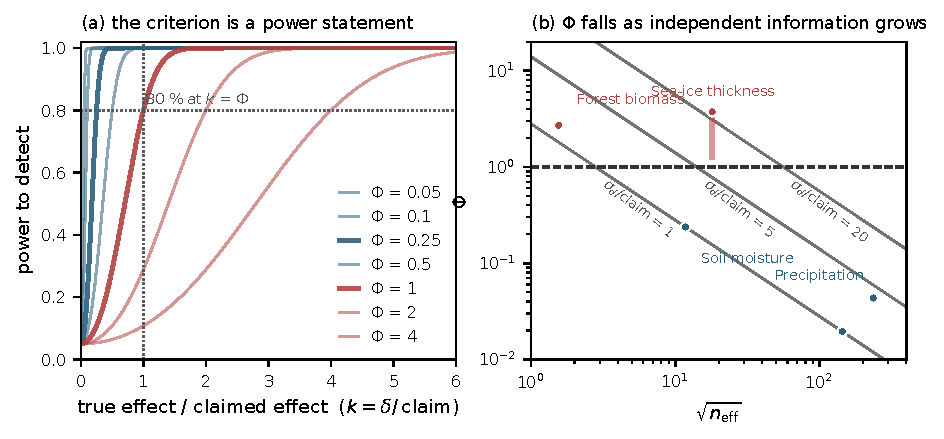
\includegraphics[width=\textwidth]{figures/fig1_power.pdf}
\caption{(a) Power to detect a true difference, expressed as a multiple $k$ of the claimed magnitude, for $\Phi$ between 0.05 and 4. The curve for $\Phi = 1$ passes through $k = 1$ at exactly 80\,\% power, which is the definition of the criterion; curves for $\Phi < 1$ reach 80\,\% at $k = \Phi < 1$, that is, below the claim, and curves for $\Phi > 1$ reach it only above the claim. (b) $\Phi$ as a function of $\sqrt{n_{\mathrm{eff}}}$ with isolines of $\sigma_d/\mathrm{claim}$ = 20, 200 and 600, with the five domains plotted; the vertical bar at $\sqrt{n_{\mathrm{eff}}} = 18$ is the sea-ice interval of Sect.~\ref{sec:kernel}.}
\label{fig:power}
\end{figure}

Figure~\ref{fig:power}a gives the same statement in the currency of the power literature: for each $\Phi$, the probability of detecting a true difference $k$ times the claim. The $\Phi = 1$ curve passes 80\,\% power at $k = 1$ by construction, the $\Phi = 0.25$ curve at $k = 0.25$; the right-hand panel places the five domains in the $(\sqrt{n_{\mathrm{eff}}}, \Phi)$ plane, separated along the axis of independent information.

\subsection{Effective sample size}

The naive count $n$ of comparisons is almost never the information content of an archive. Neighbouring flight segments share weather, nearby stations share groundwater, adjacent plots share stand structure, and successive overpasses sample the same water mass. Following the Kish design effect,
\begin{equation}
n_{\mathrm{eff}} \;=\; \frac{n^{2}}{\sum_{i}\sum_{j}\rho_{ij}},
\label{eq:kish}
\end{equation}
where $\rho_{ij}$ is the correlation between the $i$-th and $j$-th comparison errors, with $\rho_{ii}=1$. For one cluster of size $m$ with intra-cluster correlation $\rho$ this reduces to $n_{\mathrm{eff}} = n/(1+(m-1)\rho)$; for a field with correlation length $L$ over area $A$ and correlation time $\tau$ over window $T$, to $n_{\mathrm{eff}} \approx (A/2\pi L^{2})(T/\tau)$, the number of decorrelation cells. Both limits appear below; their algebra and per-domain parameters are in S1.

Equation~(\ref{eq:kish}) is the formal statement of the pseudoreplication problem \citep{hurlbert1984pseudoreplication,legendre1993spatial}, and the reason the criterion can be computed at all: $\sigma_d$ and the claim are usually reported, and $n_{\mathrm{eff}}$ can be derived from the geometry of the observing system without access to the raw archive. That derivation is an assumption, not a measurement, and the largest single source of uncertainty here; we test it with the $\pm 50\,\%$ grids of Sect.~\ref{sec:results} and S4, and for sea ice we measure it (Sect.~\ref{sec:archive} and S5).

\subsection{Properties, diagnosis and limitations}

Four properties make $\Phi$ portable: dimensionless, because $\sigma_d$ and the claim carry the same units; scale-free, since multiplying both by a constant leaves it unchanged; monotone decreasing in independent information, $\Phi \propto n_{\mathrm{eff}}^{-1/2}$, so unity requires $n_{\mathrm{eff}}\Phi^{2}$; and monotone increasing in $\sigma_d/\mathrm{claim}$, which separates the two reasons a claim can be untestable -- too few samples, or truth too coarse.

That separation is the analytical core. Sea ice fails mainly on the ratio axis -- truth is a track against a 25 km grid cell, so $\sigma_d = 0.65$ m against 2.7 cm, a ratio of 24 -- while biomass fails on both ($\sigma_d/\mathrm{claim} = 1.5$ with $n_{\mathrm{eff}} = 2.4$). Salinity and precipitation have ratios of 1.0 and 3.7 but effective sample sizes in the tens of thousands. The criterion produces a diagnosis, not merely a verdict.

Three limitations are intrinsic. Equation~(\ref{eq:mde}) uses the normal approximation; below $n_{\mathrm{eff}} \approx 20$ the non-central $t$ distribution raises the constant by 5--34\,\% (S1), which strengthens rather than weakens a $\Phi>1$ verdict. The criterion assumes a single claim; a paper making many claims should apply it to the strongest claim or adjust by false-discovery control \citep{benjamini1995controlling,storey2002direct}. And $\Phi$ presupposes that $d$ measures what the claim is about: a perfectly powered test of the wrong quantity is still the wrong test (Sect.~\ref{sec:boundary}).

\section{Inputs and provenance}
\label{sec:methods}

\subsection{Harmonisation}

Five domains are used. For each, three quantities must be placed on a common footing: $n_{\mathrm{eff}}$, $\sigma_d$ and the claim. The rule is applied identically: all three must refer to the same geophysical quantity, in the same units, averaged over the same space and time -- a claim about instantaneous 9 km soil moisture cannot be tested against daily station values, nor a basin-mean thickness claim against individual flight transects. Where a claim is phrased at a different scale we re-express it at the scale of the truth and record the transformation.

Table~S1 (S2) gives, for each domain, the raw count, the closure rule, the sources of $\sigma_d$ and of the claim, and the resulting $n_{\mathrm{eff}}$. Every entry is traceable to a peer-reviewed source or to a data product with a persistent identifier; entries that could not be traced are marked and excluded from the verdict rather than replaced by a plausible proxy. Two domains were examined and set aside on that rule: a global biomass variant, because neither the plot count nor the number of plots outside the training set could be verified, and snow depth on sea ice, because the product and the truth share the same radar.

\subsection{The five domains}

Arctic sea-ice thickness is the most intensively argued case. The product is a monthly mean field on a 25 km grid; truth consists of airborne electromagnetic and laser transects from Operation IceBridge \citep{kurtz2013sea,kurtz2011snow} and IceBird \citep{icebird_pangaea}, plus altimetry retrievals whose biases are a continuing literature \citep{laxon2013cryosat,ricker2014first,ricker2017weekly,sallila2019assessment,landy2022year}. The archive is large in files, small in information: 40\,084 granules span 338 flight days, but a sortie crosses one or two ice regimes, so capacity is set by sorties. One segment per flight day at $L = 326$ km gives 297 for 2011--2019 plus 28.2 for IceBird, hence $n_{\mathrm{eff}} = 325.2$ and a collapse factor of 123. The difference standard deviation is the one quantity measured rather than assembled: CCI against IceBird and ATM gives $\sigma_d = 0.65$ m, campaigns ranging 0.50--0.80 m. The claim is 2\,\% of the 1.36 m basin mean, 2.7 cm -- a fifth of the 0.1--0.2 m per decade basin-mean trend \citep{kwok2009thinning,laxon2013cryosat,stroeve2018arctic}.

Sea-surface salinity has the opposite geometry: the global ocean, $A = 3.6\times10^{8}$ km$^2$, decorrelation length 300--400 km \citep{vinogradova2013small,bingham2012interpolation}, decorrelation time of order three months. Truth is Argo, 13\,000 profiles per month and 1.56 million over a decade, an autonomous and repeatable system. With $L = 333$ km and $\tau = 3$ months the count is 20\,668, a collapse factor of 75. Both $\sigma_d$ and the claim are 0.20 PSU -- the former between the weekly 0.22 and monthly 0.17 of the validation literature \citep{meissner2011remote,bingham2012interpolation} -- so the ratio is 1 and $\Phi$ is driven entirely by effective sample size.

Precipitation is the best-instrumented. The Global Precipitation Climatology Centre holds 78\,000 stations, about 51\,000 reporting monthly \citep{gpcc_v2022}, and the Chinese automatic network 50\,000 daily records. With $L = 100$ km, $\tau = 3$ days, $A = 9.6\times10^{6}$ km$^2$ and $T = 1095$ days the count is 55\,768 and the collapse factor 0.90: almost every gauge is its own independent sample. The difference standard deviation is of order 3 mm d$^{-1}$, the scale of IMERG, TMPA and CMORPH intercomparisons \citep{huffman2007trmm,kidd2011status,tan2019imerg,huffman2020integrated,beck2017global,beck2019daily,sun2018review}; the claim is 20\,\% of the 4.1 mm d$^{-1}$ mean, 0.82 mm d$^{-1}$, the order of biases documented regionally \citep{li2018evaluation}. The ratio 3.7 is the second largest, yet the domain is comfortably verifiable because independent information is abundant.

Soil moisture is intermediate. The International Soil Moisture Network provides 2\,842 stations in 71 networks \citep{dorigo2011international,dorigo2021international}; the product is SMAP at 9 km \citep{entekhabi2010soil}, targeting an unbiased root-mean-square difference of 0.04 m$^3$ m$^{-3}$ \citep{colliander2017validation}. Stations within a network sample the same weather and often the same soil column, and sparse-network assimilation treats each network as roughly one degree of freedom per window \citep{gruber2018sparse}. With $m = 40$ and $\rho = 0.5$, Eq.~(\ref{eq:kish}) gives $n_{\mathrm{eff}} = 138.6$, a collapse factor of 20.5; $\sigma_d$ and the claim are both 0.04 m$^3$ m$^{-3}$, so the ratio is 1 and $n_{\mathrm{eff}}$ decides the outcome. Counting only the 18 core sites that meet the siting criteria gives $n_{\mathrm{eff}} = 18$ and $\Phi = 0.66$.

Forest biomass is the weakest case, and the only one whose truth is a set of plots. GEDI provides footprint-level aboveground biomass density \citep{dubayah2020global,duncanson2022aboveground,gedi_l4a}, calibrated against field plots and allometric models \citep{chave2014improved,saatchi2011benchmark}. In one region with 39 plots and $\rho = 0.4$, Eq.~(\ref{eq:kish}) gives $n_{\mathrm{eff}} = 2.41$, a collapse factor of 16. The difference standard deviation is 45 Mg ha$^{-1}$, the median of the published 39--94 range \citep{duncanson2022aboveground,xu2021changes,saatchi2011benchmark}; the claim is 30 Mg ha$^{-1}$, 20\,\% of a 150 Mg ha$^{-1}$ mean. Both terms are unfavourable, which is why $\Phi = 2.71$ despite a generous claim. A global variant -- about 8\,000 plots, $m = 30$, $\rho = 0.5$, $n_{\mathrm{eff}} = 516$, $\Phi = 0.18$ -- is marked not assessable because neither the plot count nor the number of plots outside the training set could be verified.

\subsection{The kernel ambiguity: why sea ice can only be an interval}
\label{sec:kernel}

One domain does not reduce to a single number, for a structural reason. The extended record supports two correlation models of the difference field, both defensible, whose floors differ by a factor of three. The first is an exponential kernel with $L = 326$ km fitted to the product's own spatial variability: 10.38 cm for the archive design with eight sorties per campaign. The second is the empirical autocorrelation of the product--truth difference itself, with $\rho(25\,\mathrm{km}) = 0.269$, $\rho(75\,\mathrm{km}) = 0.080$ and $\rho(150\,\mathrm{km}) \approx 0$; because the difference decorrelates four times faster than the field, the same archive gives 3.447 cm.

The ambiguity cannot be removed by collecting more data, and that is the point: the two kernels answer different questions, how much independent information the field contains and how much the difference contains. Which is appropriate depends on whether the claim concerns the field's representativeness or the retrieval's systematic error, and a study adopting one silently would report a floor that another equally careful study could dispute by a factor of three. We therefore treat the kernel choice as a Methods-level commitment, state both results wherever the sea-ice number appears, and report $\Phi$ as the interval spanned; the family, the design variants, the derivation and Fig.~S1 are in S3.

The complete family spans 3.40--10.38 cm; the interval quoted here, 3.447--10.098 cm ($\Phi = 1.28$--$3.74$, reported as 1.3--3.7), is the sub-family of physically realised designs, anchored to the Kish equal-weight count used for every other domain. Every member lies above the 2.7 cm claim: the verdict is kernel-independent even though the number is not.

\section{Results}
\label{sec:results}

\subsection{The five values and their ranking}

Table~\ref{tab:master} and Fig.~\ref{fig:ranking} give the result. Salinity has $\Phi = 0.019$; precipitation 0.043; soil moisture 0.24; sea-ice thickness 1.3--3.7; regional biomass 2.71. The values span more than two orders of magnitude, and the watershed falls between soil moisture and sea ice: three domains are verifiable with their existing truth archives, two are not. The sea-ice result is a statement about the archive, not the product. $\Phi$ measures the resolution the archive can bring to a claim of a given magnitude; whether a particular product's declared uncertainty is internally consistent is a separate question, and a product may be judgeable in that sense while the archive cannot resolve a sub-decimetre claim.

\begin{table}[t]
\caption{Master table. $\sigma_d$ and the claim are in the units of the domain; $\mathrm{MDE}_{80}$ is the 80\,\% verification floor in the same units; $\Phi = \mathrm{MDE}_{80}/\mathrm{claim}$. For sea ice, $\Phi$ is the interval spanned by the two correlation kernels of Sect.~\ref{sec:kernel}; the components are 1.28 (empirical difference-field autocorrelation, 3.447 cm) and 3.74 (exponential kernel, 10.098 cm). The two archive rows are the same domain under a fourteen-winter design (Sect.~\ref{sec:archive}), not additional domains: shared is the optimistic end, in which common CryoSat-2 sampling cancels in part, independent the conservative end. Neither enters the ranking.}
\label{tab:master}
\footnotesize
\setlength{\tabcolsep}{3pt}
\begin{tabular}{@{}>{\raggedright\arraybackslash}p{2.0cm}ccccc>{\raggedright\arraybackslash}p{1.7cm}@{}}
\toprule
Domain & $n_{\mathrm{eff}}$ & $\sigma_d$ & Claim & $\mathrm{MDE}_{80}$ & $\Phi$ & Verdict \\
\midrule
Sea-surface salinity & 20\,668 & 0.20 PSU & 0.20 PSU & 0.0039 PSU & 0.019 & verifiable \\
Precipitation & 55\,768 & 3.0 mm d$^{-1}$ & 0.82 mm d$^{-1}$ & 0.036 mm d$^{-1}$ & 0.043 & verifiable \\
Soil moisture & 138.6 & 0.040 m$^3$ m$^{-3}$ & 0.040 m$^3$ m$^{-3}$ & 0.0095 m$^3$ m$^{-3}$ & 0.24 & verifiable \\
Sea-ice thickness (campaign) & 325.2 & 0.65 m & 0.027 m & 0.101 m & 1.3--3.7 & not verifiable \\
Sea ice, 14-winter archive, shared & 4\,498 & 0.389 m & 0.027 m & 0.0163 m & 0.60 & verifiable$^{\dagger}$ \\
Sea ice, 14-winter archive, independent & 4\,498 & 0.65 m & 0.027 m & 0.0272 m & 1.01 & boundary \\
Forest biomass (regional) & 2.41 & 45 Mg ha$^{-1}$ & 30 Mg ha$^{-1}$ & 81.3 Mg ha$^{-1}$ & 2.71 & not verifiable \\
\bottomrule
\end{tabular}

\vspace{2pt}
{\scriptsize $^{\dagger}$Optimistic end only: CCI and CS2SMOS share the CryoSat-2 sampling, so the difference understates an independent error (Sect.~\ref{sec:archive}). At the independent end the same design gives $\Phi = 1.01$.}
\end{table}

\begin{figure}[t]
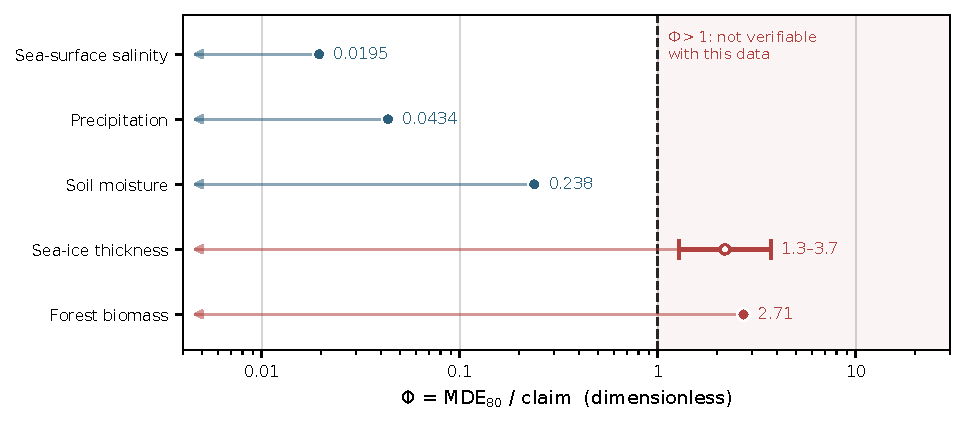
\includegraphics[width=\textwidth]{figures/fig2_ranking.pdf}
\caption{The ranking. $\Phi$ is plotted on a logarithmic axis; the dashed line is $\Phi = 1$ and the shaded region marks claims that lie below the verification floor of their archive. Sea-ice thickness is drawn as an interval because its floor depends on the correlation kernel (Sect.~\ref{sec:kernel}); the marker inside the interval is the geometric mean. Values are those of Table~\ref{tab:master}.}
\label{fig:ranking}
\end{figure}

The result is not the ranking of observational effort. Sea ice has the largest and most expensive truth archive in the set and is the least verifiable case; precipitation has the cheapest truth, a rain gauge, and is the second most verifiable. What orders them is how much independent information the archive contains per unit of asserted magnitude.

\subsection{What the criterion measures in each domain}

Figure~\ref{fig:floor} separates the two axes: claim on the horizontal, floor on the vertical, diagonals at $\Phi = 0.1$, $1$ and $10$. A domain in the lower-left triangle is verifiable; a domain above the $\Phi = 1$ line is not.

\begin{figure}[t]
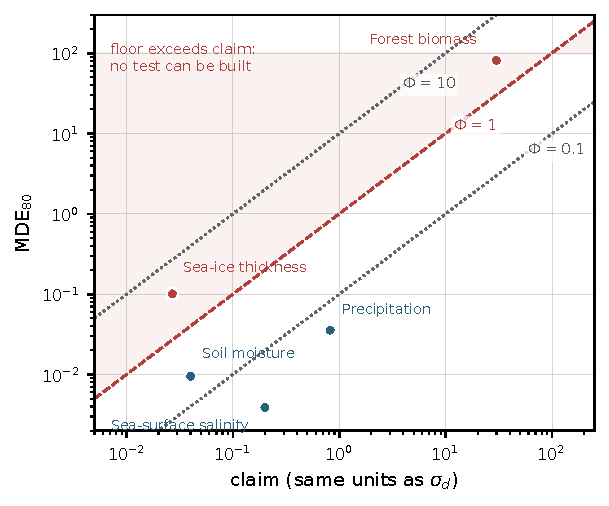
\includegraphics[width=0.62\textwidth]{figures/fig3_floor.pdf}
\caption{Verification floor against claimed magnitude, both in domain units and both on logarithmic axes. The diagonal lines are $\Phi = 0.1$, $1$ and $10$; the shaded region is the unverifiable side. Salinity and precipitation sit far below the watershed because their claims are large relative to the floor; soil moisture sits just below because its claim equals its floor but its effective sample size is 139; sea ice and biomass sit above because their floors exceed their claims.}
\label{fig:floor}
\end{figure}

Sea ice is the extreme case of the ratio axis: $\sigma_d/\mathrm{claim} = 24$, because truth is a track and the claim is about a grid cell. Its effective sample size, 325, is 135 times that of regional biomass but far from the 4\,549 needed to test a 2.7 cm bias at 80\,\% power: verification would need roughly fourteen times the independent capacity of everything flown between 2009 and 2019, or $\sigma_d$ near 0.16 m, or a claim an order of magnitude larger.

Salinity is the extreme case of the other axis: ratio 1 and floor 0.0039 PSU against a 0.2 PSU claim, so the archive could resolve a claim fifty times smaller; even one month instead of a decade, $n_{\mathrm{eff}} = 517$, leaves $\Phi = 0.12$. The domain is over-instrumented, and the question there is not whether a 0.2 PSU error can be detected but whether a smaller one can be.

Precipitation has an unusual signature: ratio 3.7, the second largest, so truth is coarse relative to the claim, yet $\Phi = 0.043$ because the collapse factor is 0.90 -- the cleanest demonstration that the axes are independent, and the reason precipitation validation can argue about 10\,\% biases \citep{beck2019daily,li2018evaluation,beck2017global} while sea-ice validation cannot.

Soil moisture is the marginal case: with $\sigma_d$ equal to the claim and $n_{\mathrm{eff}} = 138.6$, $\Phi = 0.24$; the strict 18-site closure gives 0.66 and seven independent networks would give 1.06, so the closure rule rather than the physics decides the verdict. Biomass fails for the opposite reason to sea ice: not because 45 Mg ha$^{-1}$ against a 150 Mg ha$^{-1}$ mean is coarse, but because 39 plots collapse to 2.4 samples; $\Phi = 1$ would need $n_{\mathrm{eff}} = 17.7$, about 260 plots at the same correlation, or a claim of 81 Mg ha$^{-1}$.

The $\pm 50\,\%$ grids (S4, Fig.~S2, Table~S3) separate the verdicts into three classes. Salinity, precipitation and soil moisture never approach unity, their maxima being 0.058, 0.130 and 0.714 at the corner where $\sigma_d$ is 50\,\% high and the claim 50\,\% low. Sea ice at its exponential-kernel bound never falls below unity, its minimum being 1.25. Regional biomass reaches 0.90 at the opposite corner, as does sea ice at its empirical-kernel bound (0.43). The sea-ice verdict therefore survives only under the conservative kernel, which is falsification condition F1.

\subsection{What the archive actually supplies}
\label{sec:archive}

Section~\ref{sec:criterion} treated $n_{\mathrm{eff}}$ as derivable from geometry. For sea ice it can also be measured. Subtracting the monthly CCI thickness field from CS2SMOS cell by cell wherever both are defined -- about 18\,000 of the $432\times432$ cells -- gives a monthly $\sigma_d$ whose median over the 43 overlapping winters, 2011--2024, is 0.389 m (range 0.284--0.552 m; root-mean-square 0.461 m). The same field gives the correlation structure: the empirical autocorrelation to 30 lags, with $\kappa = 1+2\sum_k\rho(k)$ truncated at the first non-positive value, gives $\kappa_x = 7.69$ and $\kappa_y = 7.07$ over 18\,033 cells in 2019-04, hence $n_{\mathrm{eff}} = 331.8$; April months give 311--394, November 150 (Figs.~S3 and S4, S5).

The measured count agrees with the design value 325.2 to 2\,\%, and that is all the agreement supports: the sortie-capacity closure is not arbitrary, but neither has the criterion been validated. What the archive changes is the verdict: fourteen winters, one independent month each, give $n_{\mathrm{eff}} = 4\,498$ and 43 pooled months 13\,816, and with the measured $\sigma_d$ the campaign $\Phi$ falls from 2.24 to 0.60, or from 3.74 to 1.006 at the independent 0.65 m. The archive reaches $\Phi<1$ at $n_{\mathrm{eff}} > 1\,631$ if $\sigma_d = 0.389$ m and at 4\,550 if $\sigma_d = 0.65$ m: the claim is not too small, the archive is too short.

Two features are carried into Table~\ref{tab:master}. CCI and CS2SMOS both ingest CryoSat-2, so a mask-related difference is common to both and cancels in part: 0.389 m is the optimistic end, 0.65 m the independent end, and the fourteen-winter verdict crosses unity between them. And $n_{\mathrm{eff}}$ has a seasonal floor -- 150 in November against 311--394 in April -- so a claim that must hold in early winter needs a longer record.

\section{Discussion}
\label{sec:discussion}

\subsection{Why a ranking is more useful than a verdict}

The most tempting reading is that geoscientific claims are generally untestable. That reading is wrong, and the five-domain design was chosen to make it wrong: three domains are comfortably verifiable, one marginally, and only one -- sea ice, the case that motivated the study -- is not. Had we examined sea ice alone we would have concluded that verification capacity is the universal bottleneck; the cross-domain comparison refutes that.

What survives is a conditional law: $\Phi > 1$ holds when truth is one-dimensional or plot-based, so $\sigma_d$ is large relative to the claim, and when independent capacity is small; it fails when truth is a dense, autonomous network that can be averaged at the product's footprint. The variable matters less than the geometry of its truth system: salinity and sea ice have almost the same decorrelation length, 333 km against 326 km, and differ by a factor of nearly 200 in $\Phi$ because one is sampled by a global array over a decade and the other by 297 spring flight days. That is more useful to a mission planner than any single verdict.

\subsection{The boundary of interpretation}
\label{sec:boundary}

$\Phi > 1$ does not mean that a study is worthless, that its data are bad, or that its authors are careless. It means that a particular quantitative claim has no test behind it in the archive as it stands. Three examples make the distinction concrete.

\citet{landy2022year} produced a year-round satellite thickness record by combining CryoSat-2 and SMOS; it resolves seasonal cycles and interannual change, and its value does not depend on whether a 2.7 cm bias can be detected. A claim about the timing of a seasonal cycle has a different magnitude and a much larger $\Phi^{-1}$. The criterion applies to claims, not to papers.

Conversely, $\Phi < 1$ does not mean that a claim is true. The Soil Moisture Active Passive mission specified 0.04 m$^3$ m$^{-3}$ \citep{entekhabi2010soil}, and core-site validation met it at 18 of 34 sites \citep{colliander2017validation}: with $\Phi = 0.24$ the archive could decide, and it decided in the negative for half the network. IMERG was reported at 0.210 mm h$^{-1}$ against a gauge reference of 0.176 mm h$^{-1}$ over China \citep{li2018evaluation}, well above the 0.82 mm d$^{-1}$-equivalent claim and far above the 0.036 mm d$^{-1}$ floor. In both cases the criterion said ``decidable'' and the decision was ``the claim fails''. Power is necessary for a verdict, not sufficient for a true one \citep{altman1995absence,greenland2016statistical}: $\Phi$ is a testability index, not a truth index.

A third failure mode is subtler: a well-powered test of the wrong quantity. If the roughly 8\,000 global biomass plots were independent of the calibration data, the closure would give $\Phi = 0.18$ and the global claim would look testable. But many of those plots are the data used to fit the GEDI models \citep{duncanson2022aboveground}, so the comparison is between a product and its own training set. The effective sample size is then not small; it is undefined in the intended sense, and no arithmetic rescues it. An index computed from a leaky truth is worse than no index at all, which is why that variant is marked not assessable in Table~S1.

\subsection{Relation to existing frameworks}

The criterion is a composition of established pieces. The numerator is the minimum detectable effect of the power literature \citep{cohen1992power,lenth2001some,nakagawa2007effect}, inverted so that the effect is given and the required sample size is the question; the denominator's square root is the Kish design effect, whose spatial and temporal forms are the effective-degrees-of-freedom machinery of climate diagnostics \citep{bretherton1999effective,zwiers1995taking,kunsch1989jackknife,politis1994stationary}, with the pseudoreplication warning as its ecological counterpart \citep{hurlbert1984pseudoreplication,legendre1993spatial,dutilleul1993modifying}. The validation-practice literature supplied the vocabulary of product--truth comparison \citep{loew2017validation,merchant2017uncertainty,taylor2001summarizing}.

What is new is not any ingredient but the ratio and its uses. Validation studies report error metrics and mission requirements are stated as accuracy targets, both silent on whether the two are commensurate; $\Phi$ makes the comparison explicit and dimensionless, so a sea-ice paper and a soil-moisture paper share an axis. It also makes the design question quantitative: ``we need $\Phi^{2}$ times more independent truth'' is a budget line, not a caveat. And it complements multiple-testing control, addressing not the claim accepted too readily but the claim that could never have been rejected \citep{benjamini1995controlling,storey2002direct}.

\subsection{Falsification conditions}
\label{sec:falsification}

The conclusions are testable; each of the following observations would require them to be revised, and each is stated with the threshold that would trigger the change.

F1. A defensible measurement of $\sigma_d$ for monthly gridded sea-ice thickness near 0.30 m rather than 0.65 m would bring the exponential-kernel $\Phi$ to 1.73 and the empirical-kernel $\Phi$ to 0.59. The sea-ice verdict would become kernel-conditional and the headline interval would have to be withdrawn.

F2. A demonstration that the empirical difference-field autocorrelation is the appropriate kernel for bias claims -- for instance that the product's systematic error decorrelates at 25--75 km while its representativeness error does not -- would move the sea-ice $\Phi$ to 1.28 and, with F1, below unity.

F3. A verified count of at least 500 independent, non-training global biomass plots, with the stated 45 Mg ha$^{-1}$ $\sigma_d$, would give $\Phi = 0.18$ for the global claim and remove biomass from the unverifiable class; the regional verdict would stand.

F4. A re-derivation of the soil-moisture closure putting independent information below 8 samples -- for example seven networks rather than 71 -- would raise $\Phi$ above 1 and move soil moisture across the watershed.

F5. A salinity requirement below 0.0039 PSU, or a precipitation requirement below 0.036 mm d$^{-1}$, would move those domains from verifiable to unverifiable. No such requirement exists, which is itself evidence that both are claim-limited rather than archive-limited.

F6. A demonstration that the 2.802 constant is inappropriate because validation claims are one-sided would lower the floor by 11\,\% ($z_{0.95}+z_{0.80} = 2.486$); sea-ice $\Phi$ would become 1.12--3.32 and no verdict would change, so the choice of constant, unlike the choice of kernel, is robust.

\subsection{Limitations}

Four limitations deserve statement. Four of the five $\sigma_d$ values are literature-based; only the sea-ice value was computed from a difference field, and the $\pm 50\,\%$ grids are the response: the three verifiable domains are insensitive, the two unverifiable ones are not. The closure rules are assumptions -- the sortie-capacity rule for sea ice and the cluster rule for biomass mattering most -- and both are stated with their parameters so that a reader who disagrees can recompute. The normal approximation and a fixed 80\,\% power are conventions, and S1 shows how the numbers change under alternatives. And one claim at a time is evaluated: a paper claiming a bias, a variance and a trend has three values of $\Phi$.

The archive measurement adds two limitations. Common-mode cancellation, as above, makes 0.389 m optimistic and 0.65 m the independent end, and the verdict is reported at both. The measured $n_{\mathrm{eff}}$ is one input checked against an independent construction, not a validation of the criterion; the 2\,\% agreement supports only the claim that the design count is not arbitrary. Neither limitation changes the five-domain ranking, which uses the campaign design and the airborne $\sigma_d$; both bear on any reading of the archive rows of Table~\ref{tab:master} as evidence that a 2.7 cm bias has become verifiable.

\section{Conclusions}

A claim can be false, true, or untestable, and the third category is invisible in most model-assessment reporting. This paper makes it visible with a single dimensionless number. $\Phi = 2.802\,\sigma_d/(\mathrm{claim}\sqrt{n_{\mathrm{eff}}})$ compares the minimum difference an archive can resolve at 80\,\% power with the difference a claim asserts, and returns a value above unity when the claim lies below the floor. It changes no retrieval, no model and no archive, and requires only three numbers an assessment already reports.

Applied to five domains with published truth archives and accuracy claims, the criterion orders them: salinity 0.019, precipitation 0.043, soil moisture 0.24, sea-ice thickness 1.3--3.7, regional biomass 2.71. Three can test the claims they make; two cannot. The ordering is driven by the geometry of the truth system rather than its cost or the geophysical variable, and it is the cross-domain comparison, not any single value, that carries the content.

Sea-ice thickness is the case in which the floor itself is not a single number. Two defensible kernels give 3.447 cm and 10.38 cm, a factor of 2.5 between their optima and 3.0 at fixed design; the interval is reported, the ambiguity treated as a Methods-level commitment, and the verdict shown to be kernel-independent because every member exceeds the 2.7 cm claim. Under a $\pm 50\,\%$ perturbation the three verifiable domains stay verifiable and sea ice stays unverifiable at its conservative bound, while regional biomass and the empirical-kernel bound cross unity at the optimistic corner -- crossings reported as falsification conditions rather than smoothed away.

The criterion is necessary but not sufficient: it says a claim can be decided, not that it is right, since the SMAP claim has $\Phi = 0.24$ and was met at 18 of 34 sites and IMERG's Chinese bias exceeds its floor by a wide margin. Used with that boundary in mind, $\Phi$ turns ``more validation is needed'' into an arithmetic statement about how much more, of what kind, and whether the present claim could ever have been checked.

\section*{Code and data availability}

The example implementation, the input table and the derived tables are archived with the paper and mirrored in a public code repository, \url{https://github.com/dddsx3/free-demo}. The archive is to be deposited in a persistent public repository (Zenodo or an institutional equivalent); a DOI is deliberately not asserted in this draft, because none has been minted, and the placeholder \texttt{[DOI: ZENODO-TO-BE-\allowbreak ASSIGNED]} must be replaced before submission. The implementation was run with Python 3.14.2, NumPy 2.4.1, SciPy 1.17.0 and pandas 3.0.0; Matplotlib 3.10.8 is used for the figures. From the repository root, \texttt{python code/\allowbreak run\_all.py} executes the full chain (arithmetic, number check, figures, both PDFs) and \texttt{python code/\allowbreak run\_all.py --refs} adds the DOI re-resolution. An optional stage reproduces the worked example of S7: \texttt{python code/\allowbreak run\_all.py --archive --p1 <dir>}, or \texttt{python code/\allowbreak archive\_example.py --p1 <dir>} alone, reads two monthly product fields from outside this archive and writes \texttt{data/archive/}. It is optional because those fields are not redistributed here. Nine regression tests in \texttt{code/\allowbreak test\_phi\_core.py}, run with \texttt{python -m pytest code}, check that the five $\Phi$ values, the three closure identities and the integral-scale rule still reproduce this manuscript. The chain writes seven derived tables and the three committed archive tables that Figs.~S3 and S4 read, and seven figures, four of which appear in the supplement; the inventory is in S7 and in \texttt{REPRO\_CHECK.txt}. The script exits non-zero if a headline number moves by more than 0.1\,\% from the value printed here. No observational granule is downloaded; the truth archives are cited in Table~S1 and carry their own persistent identifiers.

\section*{CRediT authorship contribution statement}

[AUTHOR CONTRIBUTION STATEMENT]

\section*{Declaration of competing interest}

[COMPETING INTERESTS STATEMENT]

\section*{Acknowledgements}

[AUTHOR ACKNOWLEDGEMENTS]

\bibliographystyle{elsarticle-harv}
\bibliography{refs}

\end{document}
